\chapter{Introdu��o}

Em m�todos num�ricos para obter solu��es aproximadas de equa��es diferenciais,
tais como o m�todo dos elementos finitos (MEF)\abbrev{MEF}{m�todo de elementos
finitos} e o m�todo dos volumes finitos (MVF)\abbrev{MVF}{m�todo de volumes
finitos}, o dom�nio no qual estas equa��es foram definidas � discretizado em
sub-dom�nios simples denominados \textit{elementos}.

Denotemos o dom�nio por $\Omega$\symbl{$\Omega$}{dom�nio de defini��o de uma
equa��o diferencial}. Seja $\partial \Omega$ o contorno de
$\Omega$.\symbl{$\partial$}{operador do contorno.}

\section{Motiva�{\~ a}o}
adsadsda

\begin{figure}[ht]
\centering
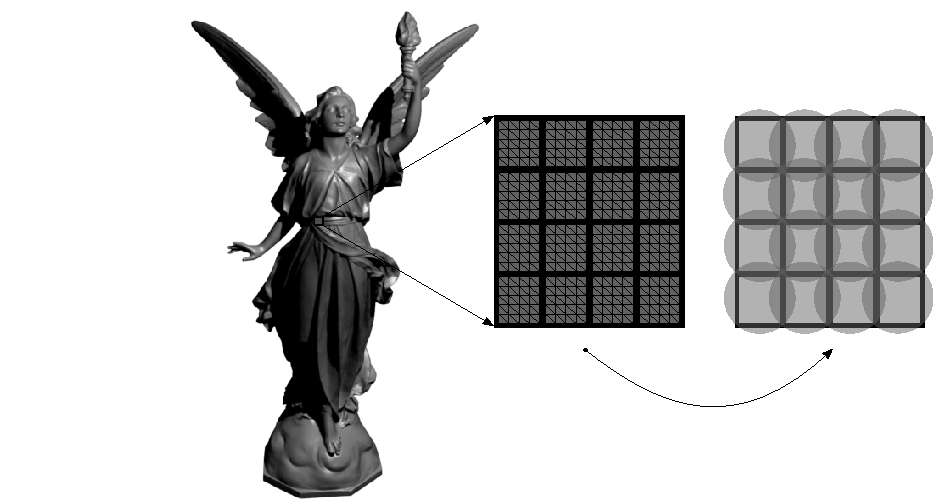
\includegraphics[width=8.0cm,bb = 0 0 100 100]{lucyIo} 
\caption{Merging splats}
\label{fig:merge}
\end{figure}

\subsection{ASdasdsad}
adasda

\section{Objetivo}

\section{Metodologia}

\section{Organiza�{\~ a}o da tese}
